\documentclass[11]{article}

\usepackage[a4paper,left=3cm,right=2cm,top=2.5cm,bottom=2.5cm]{geometry}
\usepackage{lipsum}
\usepackage{amsmath}
\usepackage{multirow}	
\usepackage{graphicx}


\title{Machine Learning HW1}
\author{Payam AZAD - 503111554}
\begin{document}
\pagenumbering{gobble}
 \maketitle
 
 \begin{table}[ht!]
\centering
\label{my-label}
\begin{tabular}{|ll|l|l|l|l|l|l|}
\hline
                                             &          & Q1 & Q2 & Q3 & Q4 & Q5 & Total \\ \hline
\multicolumn{1}{|l|}{\multirow{2}{*}{Grade}} & Max      & 1  & 1  & 1  & 1  & 1  & 5     \\ \cline{2-8} 
\multicolumn{1}{|l|}{}                       & Expected & 1  & 1  & 1  & 1  & 1  & 5     \\ \hline
\end{tabular}
\end{table}


 \section*{Q1}
 \subsection*{Q1a}
 $P(X=1|Y=0) = \frac{P(X=1,Y=0)}{P(Y=0)} = \frac{0.20}{0.15 + 0.3 + 0.2} = 0.307$
 \subsection*{Q1b}
 consider: \\
 $P(X=1) = 0.05 + 0.2 = 0.25$ \\
 $P(x=1) \neq P(X=1 | Y=1)$ \\
 so it is not independent.
 \subsection*{Q1c}
 $E[5*X + 3*Y*Y] = 5E[X] + 3E[Y^2]$
 \section*{Q3}
we are trying to find: 
$p(terrorist=true | detected=true)$ \\
that is : \\
$p(terrorist=true | detected=true) = \frac{p(detected=true | terrorist=true) p(terrorist=true ) }{p(detected=true) }$ \\
$p(detected=true | terrorist=true) = 0.95$ \\
$p(terrorist=true ) = 0.01$ \\
$p(detected=true) = p(detected=true∣terrorist=true)p(terrorist=true)+p(detected=true∣terrorist=false)p(terrorist=false)$ 
$=0.95(0.01)+0.05(0.99)=0.059$ \\
$p(terrorist=true | detected=true) = \frac{0.95 * 0.01}{0.059} = 0.161$


 \section*{Q4}
we need to choose i that has the maximum result for : $EU(\alpha_i|x) = \displaystyle\sum_{k} U_{ik}P(S_k|x)$ \\
we have: \\
$EU(\alpha_1|x) = 5 * 0.7 + 3 * 0.2 + 1 * 0.1 = 4.2$\\
$EU(\alpha_2|x) = 0 * 0.7 + 4 * 0.2 + -2 * 0.1 = 0.6$\\
$EU(\alpha_3|x) = -3 * 0.7 + 0 * 0.2 + 10 * 0.1 = -1.1$\\
so the best decision is $i = 1$

 \section*{Q5}
 \subsection*{Q5a} 

 
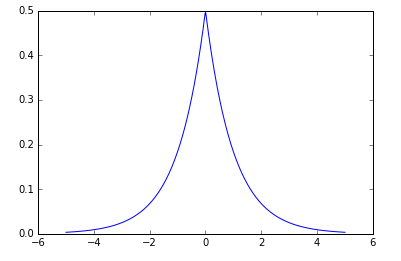
\includegraphics[scale=0.5]{fig1.png}
\\\\
 $p(x > 2) = \int_2^\infty \frac{1}{2}\mathrm{e}^{-|x|}\,\mathrm{d}x = \int_2^\infty \frac{1}{2}\mathrm{e}^{-x}\,\mathrm{d}x$ \\
 $ = -0.5 * (0 - e^{-2}) = 0.0676$

 \subsection*{Q5b}
 \begin{align*}
E[x] = \sum^n_{k=0}k\binom nkp^k(1-p)^{n-k}&=\sum_{k=0}^nn\binom{n-1}{k-1}p^k(1-p)^{n-k}\\
&=n\sum_{k=0}^n\binom{n-1}{k-1}p^k(1-p)^{n-k}\\
&=n\sum_{k=0}^{n-1}\binom{n-1}kp^{k+1}(1-p)^{n-k-1}\\
&=np\sum_{k=0}^{n-1}\binom{n-1}kp^k(1-p)^{n-k-1}\\
&=np\Big(p+(1-p)\Big)^{n-1}\\
&=np\
\end{align*}
\begin{align*}
E[x^2] = E[X(X-1)]+E[X] = n(n-1)p^2 + np
\end{align*}
 \\\\\\
 

\end{document}